\chapter{Wigner関数}
\section{Winger表示}
\subsection{定義}
Wigner関数の定義は以下の通り:
\begin{eqnarray}
  f_W(q, p, t) = \frac{1}{2\pi\hbar}\int_{-\infty}^{\infty} ds \bra{q-\frac{s}{2}}\ket{\psi(t)}\bra{\psi(t)}\ket{q+\frac{s}{2}}e^{ips/\hbar}\label{wigner1}
\end{eqnarray}
もしくは
\begin{eqnarray}
  f_W(q, p, t) = \int_{-\infty}^{\infty} d\overline{q}_{12} \bra{q_1}\ket{\psi(t)}\bra{\psi(t)}\ket{q_2}e^{-ip\overline{q}_{12}/\hbar}\label{wigner2}
\end{eqnarray}
とすることもできる. ここでは$q_{12} = (q_1 + q_2)/2$, $\overline{q}_{12} = q_1 - q_2$である.
\begin{comment}
  以下では(\ref{wigner})の流儀を採用することにする.
\end{comment}
\subsection{任意の演算子に対するWigner表示}
任意の演算子$\hat{A}$に対するWigner表示は
\begin{eqnarray}
  A_W(q_{12}, p) = \int_{-\infty}^{\infty} d\overline{q}_{12} \bra{q_1}\hat{A}\ket{q_2}e^{-ip\overline{q}_{12}/\hbar}\label{wigner_op}
\end{eqnarray}
である. ここで
\begin{eqnarray}
  \bra{q_1}\hat{A}\ket{q_2} = \frac{1}{2\pi}\int dp A_W(q_{12}, p)e^{-ip\overline{q}_{12}}\label{wigner_formula}
\end{eqnarray}
が成立している.
\section{Wigner分布関数の時間発展}
$f_W(q, p, t)$の時間発展方程式を導く. その準備として2つの演算子同士の積($\hat{A}\hat{B}$)のWigner変換がどのように計算できるかを考える. 
\subsection{$(\hat{A}\hat{B})_W$の計算}
今回は式(\ref{wigner1})の流儀を採用する:
\begin{eqnarray}
  (\hat{A}\hat{B})_W &=& \int_{-\infty}^{\infty}ds \bra{q-\frac{s}{2}}\hat{A}\hat{B}\ket{q+\frac{s}{2}}e^{ips/\hbar}
  = \int_{-\infty}^{\infty}\int_{-\infty}^{\infty}ds dq' \mel**{q-\frac{s}{2}}{\hat{A}}{q'}\mel**{q'}{\hat{B}}{q+\frac{s}{2}}e^{ips/\hbar}\label{wigner_start}
\end{eqnarray}
ここで式(\ref{wigner_formula})を用いて変形する:
\begin{eqnarray}
  \frac{1}{(2\pi\hbar)^2}\int ds dq' dp' dp'' e^{ips/\hbar}e^{-ip'\qty(q-q'-\frac{s}{2})/\hbar} e^{-ip''\qty(q'-q-\frac{s}{2})/\hbar}A_W\pqty{\frac{q+q'}{2} - \frac{s}{4}, p'}B_W\qty(\frac{q+q'}{2} + \frac{s}{4}, p'')
\end{eqnarray}
expの肩の変数に着目して$A_W, B_W$の変数を変形する:
\begin{eqnarray}
  \nonumber\frac{1}{(2\pi\hbar)^2}\int ds dq' dp' dp'' &&e^{ips/\hbar}e^{-ip'\qty(q-q'-\frac{s}{2})/\hbar} e^{-ip''\qty(q'-q-\frac{s}{2})/\hbar}\\
 && \times A_W\qty(q + \frac{1}{2}\pqty{q'-q-\frac{s}{2}}, p')B_W\qty(q - \frac{1}{2}\pqty{q-q'-\frac{s}{2}}, p'')
\end{eqnarray}
これを並進演算子を用いて
\begin{eqnarray}
  \nonumber\frac{1}{(2\pi\hbar)^2}\int ds dq' dp' dp'' &&e^{ips/\hbar}e^{-ip'\qty(q-q'-\frac{s}{2})/\hbar}e^{-ip''\qty(q'-q-\frac{s}{2})/\hbar}\\
  &&\times\qty(e^{\frac{1}{2}\pqty{q'-q-\frac{s}{2}}\partial_q}A_W\qty(q, p'))\qty(e^{-\frac{1}{2}\pqty{q-q'-\frac{s}{2}}\partial_q}B_W\qty(q, p''))
\end{eqnarray}
と変形. さらに並進変換$e^{a\partial_q}e^{pq} = e^{p(q+a)}$を用いて
\begin{eqnarray}
  \nonumber\frac{1}{(2\pi\hbar)^2}\int&& ds dq' dp' dp'' e^{ips/\hbar}\\
  &&\times\qty(A_W\qty(q, p')e^{\frac{i\hbar}{2}\overleftarrow{\partial}_q\overrightarrow{\partial}_{p''}}e^{-ip''\qty(q'-q-\frac{s}{2})/\hbar})\qty(e^{-ip'\qty(q-q'-\frac{s}{2})/\hbar}e^{-\frac{i\hbar}{2}\overleftarrow{\partial}_{p'}\overrightarrow{\partial}_{q}}B_W\qty(q, p''))
\end{eqnarray}
とする. ここで$\overleftarrow{\partial}, \overrightarrow{\partial}$はそれぞれ左側, 右側に作用する演算子である. 次に$q'$の積分を計算する:
\begin{eqnarray}
  \nonumber\frac{1}{2\pi\hbar}\int&& ds dp' dp'' e^{ips/\hbar}\\
  &&\times\qty(A_W\qty(q, p')e^{\frac{i\hbar}{2}\overleftarrow{\partial}_q\overrightarrow{\partial}_{p''}}e^{i(p'-p'')q/\hbar}\delta(p''-p')e^{-\frac{i}{2}(p''+p')s/\hbar}e^{-\frac{i\hbar}{2}\overleftarrow{\partial}_{p'}\overrightarrow{\partial}_{q}}B_W\qty(q, p''))
\end{eqnarray}
$p''$で積分:
\begin{eqnarray}
  &&\frac{1}{2\pi\hbar}\int ds dp' e^{ips/\hbar}\qty(A_W\qty(q, p')e^{\frac{i\hbar}{2}\overleftarrow{\partial}_q\overrightarrow{\partial}_{p'}}e^{-ip's/\hbar}e^{-\frac{i\hbar}{2}\overleftarrow{\partial}_{p'}\overrightarrow{\partial}_{q}}B_W\qty(q, p'))\\
  &=& \frac{1}{2\pi\hbar}\int ds dp' \qty(A_W\qty(q, p')e^{\frac{i\hbar}{2}\overleftarrow{\partial}_q\overrightarrow{\partial}_{p'}}e^{i(p-p')s/\hbar}e^{-\frac{i\hbar}{2}\overleftarrow{\partial}_{p'}\overrightarrow{\partial}_{q}}B_W\qty(q, p'))
\end{eqnarray}
$s$で積分:
\begin{eqnarray}
  \int dp' \qty(A_W\qty(q, p')e^{\frac{i\hbar}{2}\overleftarrow{\partial}_q\overrightarrow{\partial}_{p'}}\delta(p-p')e^{-\frac{i\hbar}{2}\overleftarrow{\partial}_{p'}\overrightarrow{\partial}_{q}}B_W\qty(q, p'))
\end{eqnarray}
最後に$p'$で積分:
\begin{eqnarray}
  \qty(A_W\qty(q, p)e^{\frac{i\hbar}{2}\overleftarrow{\partial}_q\overrightarrow{\partial}_{p}}e^{-\frac{i\hbar}{2}\overleftarrow{\partial}_{p}\overrightarrow{\partial}_{q}}B_W\qty(q, p))
\end{eqnarray}
つまり, $e^{\frac{i\hbar}{2}\qty(\overleftarrow{\partial}_q\overrightarrow{\partial}_{p}-\overleftarrow{\partial}_{p}\overrightarrow{\partial}_{q})} = e^{\frac{i\hbar}{2}\Lambda}$とおくと,
\begin{eqnarray}
  (\hat{A}\hat{B})_W = A_W(q, p)e^{\frac{i\hbar}{2}\Lambda}B_W(q, p)\label{wigner_end}
\end{eqnarray}
\subsection{$f_W(q, p, t)$の時間発展}
以上の結果を基に$f_W(q, p, t)$の時間発展方程式を導く. Schr\"odinger方程式
\begin{eqnarray}
  i\hbar\partial_t\ket{\psi(t)} = \hat{H}\ket{\psi(t)}
\end{eqnarray}
を用いて, 式(\ref{wigner2})の時間微分は以下のようにまとめられる:
\begin{eqnarray}
  i\hbar\partial_tf_W(q, p, t) &=& \int_{-\infty}^{\infty} d\overline{q}_{12} \bra{q_1}\qty(i\hbar\partial_t\ket{\psi(t)}\bra{\psi(t)})\ket{q_2}e^{-ip\overline{q}_{12}/\hbar}\\
  \nonumber  &=& \int_{-\infty}^{\infty} d\overline{q}_{12} \bra{q_1}(i\hbar\partial_t\ket{\psi(t)})\bra{\psi(t)}\ket{q_2}e^{-ip\overline{q}_{12}/\hbar}\\
  &&\hspace{0.5cm} + \int_{-\infty}^{\infty} d\overline{q}_{12} \bra{q_1}\ket{\psi(t)}(i\hbar\partial_t\bra{\psi(t)})\ket{q_2}e^{-ip\overline{q}_{12}/\hbar}\\
  &=& \int_{-\infty}^{\infty} d\overline{q}_{12} \mel**{q_1}{\comm{\hat{H}}{\ket{\psi(t)}\bra{\psi(t)}}}{q_2}e^{-ip\overline{q}_{12}/\hbar}\\
  &=& (\hat{H}\ket{\psi(t)}\bra{\psi(t)})_W - (\ket{\psi(t)}\bra{\psi(t)}\hat{H})_W\\
  &=& H_W(q, p)e^{\frac{i\hbar}{2}\Lambda}f_W(q, p, t) - f_W(q, p, t)e^{\frac{i\hbar}{2}\Lambda}H_W(q, p)\label{wigner-moyal}
\end{eqnarray}
\section{具体的な問題}
以上の定式化を具体的なモデルに落とし込み, 数値計算で相空間上の運動を見る.
\subsection{調和振動子系のWigner-Moyal方程式}
ハミルトニアンを
\begin{eqnarray}
  \hat{H} = \frac{\hat{p}^2}{2m} + \frac{1}{2}m\omega^2\hat{q}^2
\end{eqnarray}
とする. このハミルトニアンのWigner表示は
\begin{eqnarray}
  H_W(q, p) = \frac{p^2}{2m} + \frac{1}{2}m\omega^2q^2
\end{eqnarray}
である. これを(\ref{wigner-moyal})に代入:
\begin{eqnarray}
  i\hbar\partial_tf_W(q, p, t) = \qty(\frac{p^2}{2m} + \frac{1}{2}m\omega^2q^2)e^{\frac{i\hbar}{2}\Lambda}f_W(q, p, t) - f_W(q, p, t)e^{\frac{i\hbar}{2}\Lambda}\qty(\frac{p^2}{2m} + \frac{1}{2}m\omega^2q^2)
\end{eqnarray}
これを計算する. 面倒なので以下では$m = \omega = \hbar = 1$の単位系を採用.  
\begin{eqnarray}
  \partial_t f_W(q, p, t) = \qty(q\partial_p - p\partial_q)f_W(q, p, t)\label{wigner-moyal2}
\end{eqnarray}
のような偏微分方程式が導出される. これを数値的に解きたい.
\subsection{数値計算}
\subsubsection{差分化}
今回は簡単のため, 普通に差分化する. 差分化した方程式はMoyal方程式は
\begin{eqnarray}
  f(t_{n+1}) = k_1\qty[q_lf(p_{m+1}) - p_mf(q_{l+1})] + \qty[k_1(-q_l + p_m) + 1]f
\end{eqnarray}
となる. ここでいくつかの記号の省略ルールを示す:
\begin{itemize}
\item Wigner表示の添字$W$は省略
\item $f(q_l, p_m, t_n)$のように差分化しており, $q, p$の幅は$h_{qp}$, $t$の幅は$h_t$.
\item $f(q_l, p_m, t_n) \rightarrow f$, $f(q_{l+1}, p_m, t_n) \rightarrow f(q_{l+1})$などの表記を用いている.
  \item $h_t/h_{qp} = k_1$.
\end{itemize}
これで数値計算が可能な形になった.
\subsubsection{問題点}
上の差分化は単なる前進差分なので${\cal O}(h_{qp}), {\cal O}(h_{t})$の誤差を生じる. これで計算すると, よほど細かく差分化しないとヤバいです. 誤差が累積して襲ってきます. せめて中央差分にしましょう. 
\subsubsection{初期条件}
%% 初期関数として
%% \begin{eqnarray}
%%   f_0 = \sqrt{\frac{5}{\pi}}e^{5(q+\frac{1}{2})^2}
%% \end{eqnarray}
%% を用意する(やる気なさ過ぎ?).
あるガウス波束$f_0$のWigner表示として
\begin{eqnarray}
  f_{0W} = \frac{1}{\pi}e^{-(q+4)^2 -p^2}\label{harmonic_wigner}
\end{eqnarray}
を用意する.$f_0$はこんなかんじ:
\begin{figure}[htbp]
  \centering
  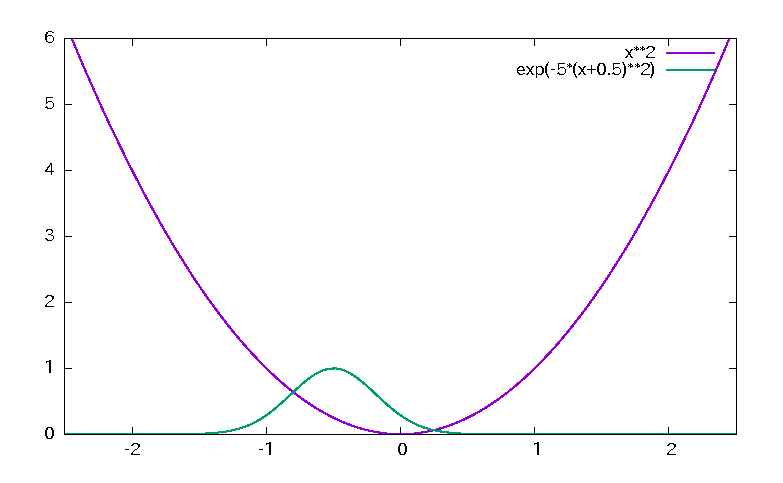
\includegraphics[width = 7cm]{./EPS/wave_packet.eps}
  \label{fig1}
\end{figure}
\\
この波束が調和型トラップによって振動する. 古典粒子が調和振動子トラップ内で振動するとき, 位相空間上の点は楕円を描くように動くはずでありWigner関数も同様の動きをするが, 相空間上では$q, p$方向の広がりがある. 
\begin{figure}[htbp]
  \begin{center}
    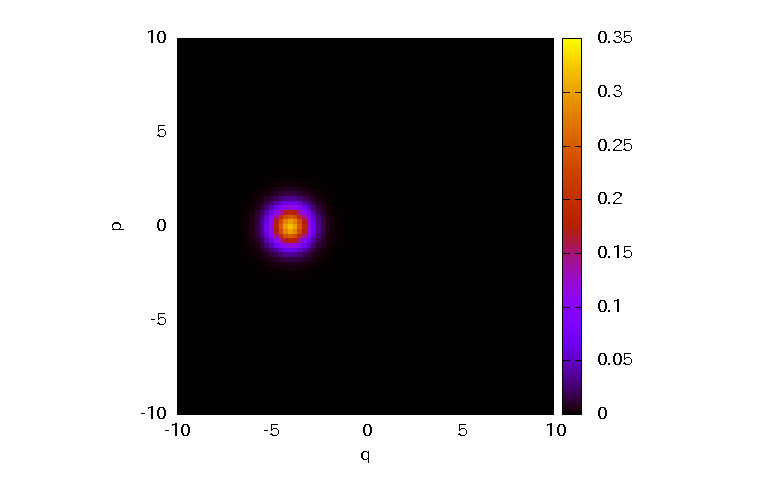
\includegraphics[width = 12cm]{./EPS/wigner_function.eps}
  \end{center}
  \label{fig2}
\end{figure}\\
こんなほんやりした玉みたいなのが位相空間上をぐるぐる回るはず. 

